\chapter{\;\;\;\;Overview}\label{sec:overview}

%% \jeehoon{In title, maybe no space before colon?}

Modern software systems are complex, and modularity is the crucial tool for coping with such complexity.
That is, software systems are typically broke up into multiple modules so that software developers can focus on a single module at a time.
Moreover, instead of directly writing each module in assembly, they are mostly written in high-level languages such as C.
Then compilers translate such high-level languages into assembly via multiple translation passes.




To verify such a system end-to-end, it is critically important to have a modular verification technique.
Specifically, the verification can be divided into two parts, compiler verification and program verification,
where the former is about proving the generated assembly code behaves as specified by the semantics of the source program,
and the latter is about proving desired properties about the behaviors of the source program.
In compiler verification, we want to focus on a single compiler and its single translation at a time, even though each modules are written in different languages and compiled with different compilers.
Similarly, in program verification, we want to focus on a single module and its single abstraction at a time, assuming interfaces of other modules.




However, none of the existing approaches are satisfactory.
For compiler verification, there are two state-of-the-art frameworks, \ccx{} \cite{gu:dscal,wang:saccx} and Compositional CompCert (shortly, \ccc{}) \cite{beringer:isem,stewart:ccc},
supporting modular verification of multi-language systems. %heterogeneous systems.
The former simplifies the problem by
imposing restrictions that the source modules should have no mutual
dependence and be verified against certain well-behaved
specifications. On the other hand, the latter develops a new
verification technique that directly solves the problem but at the
expense of significantly increasing the verification cost.
For program verification, higher-order separation logic (such as VST\cite{VST}) has shown great success, but it also has shortcomings:
its underlying model (and thus soundness result) is esoteric, it proves partial correctness instead of total correctness,
and its soundness theorem is applicable only when the whole program is verified with the same logic.
%does not support gradual abstraction.








In this dissertation, we develop a novel modular verification technique, called RUSC (Refinement
Under Self-related Contexts) (\Cref{sec:rusc}), and demonstrate its usefulness by applying it to
both compiler verification (\Cref{sec:compiler}) and program verification (\Cref{sec:program}).
%% Specifically, RUSC solves the problem without aforementioned restrictions but still with low verification overhead.
Specifically, we develop CompCertM, a full
extension of the latest version of CompCert supporting multi-language
linking, and show how RUSC enables modular compiler verification without any restrictions but still with low verification overhead.
Moreover, we verify interesting programs using RUSC as a program logic, and demonstrate that it does not suffer from aforementioned drawbacks of higher-order separation logic.
Although the result shows potential, RUSC-as-a-program-logic is still on its early stage and we discuss future research directions.
%% Moreover, we demonstrate the power of RUSC as a program
%% verification technique by modularly verifying interesting programs
%% consisting of C and handwritten assembly against their mathematical
%% specifications.
%% Compared to higher-order separation logic, our approach does not suffer from aforementioned drawbacks, but 
%%% %has clearer specification, supports full functional correctness, and allows gradual abstraction,
%% but its verification overhead is relatively high.
%%We leave it as future work to adopt the core ideas and automation from higher-order separation logic to lower the verification overhead.

%% \paragraph{\Cref{sec:rusc}: RUSC theory}
%% \paragraph{\Cref{sec:compiler}: Compiler Verification: CompCertM}
%% \paragraph{\Cref{sec:program}: Program Verification}

This dissertation draws heavily on the work and writing in the following paper: \cite{song:compcertm}

\section{Compiler Verification}\label{sec:overview:compiler}
\cc{} \cite{CompCert, Compcert-CACM}, the first \emph{verified}
\emph{optimizing} compiler for \emph{the C programming language}, has
served as a backend in end-to-end verified
software~\cite{appel2014program}. Specifically, \cc{} compiles programs written in (a
large subset of) C down to assembly code via various translation
passes including a number of common optimizations.  Moreover, it is
formally verified in Coq that every translation of \cc{} preserves the
semantics: the generated assembly code behaves as specified by the
semantics of the source program. Therefore, \cc{} has been used to
transform verification results about the source C program into those
about the compiled assembly code in various projects such as
CertiKOS~\cite{CertiKOS11, CertiKOS16} and VST~\cite{VST}.

There is, however, a limitation in the original \cc{} that restricts
its application to a more wide range of software verification---namely
the lack of support for handwritten assembly. This
limitation can be serious in verification of \emph{real-world}
software because handwritten assembly is often crucial for writing
low-level system software or library code.

To overcome this limitation, two extensions of \cc{}, namely \ccx{}
\cite{gu:dscal,wang:saccx} and Compositional CompCert (shortly, \ccc{}) \cite{beringer:isem,stewart:ccc}, have
been developed. Interestingly, they take different approaches to
\emph{two key challenges}:
\begin{enumerate}
\item how to modularly verify each translation of each
module using a different relational memory invariant (shortly, memory relation) and compose the proofs all
together; and
\item how to deal with illegal interference from
arbitrary (handwritten) assembly modules that can invalidate compiler
translations of C modules (\eg not preserving the
callee-save register values).
\end{enumerate}

\revision{%
We elaborate more on the first, more fundamental, challenge.
\cc{} uses three different memory relations called memory \emph{identity},
\emph{extension} and \emph{injection} (in the order of complexity and generality)
for a proof engineering purpose: it uses a
simpler relation whenever possible to simplify the correctness proof.
%
The challenge occurs in an open setting where a translation of an
open module is verified separately. In a closed setting as in \cc{}
where the whole closed program (\ie all the modules) is compiled by the
same translation pass thereby being verified as a whole,
verification of such a closed program using a simpler relation essentially implies
that using a more general one.  However, in an open setting (\ie for
verification of an open module), that implication does not hold
because such verification assumes that the unknown contexts also
preserve the same memory relation. In other words, using a simpler
relation, the verification guarantees a stronger property on its own
module but assumes a stronger property on the context modules.
Therefore, verification of open modules using different memory relations
cannot be compared, which makes composition of such verifications hard.%
}

\myparagraph{\ccx{}'s Approach}
%
\ccx{} is developed as a backend compiler for the verified OS kernel
\certikos{} \cite{CertiKOS11,CertiKOS16} and thus specialized for this purpose.
Specifically, \ccx{} simplifies the two challenges by making two
assumptions that $(i)$ there are no mutual dependencies among the
input modules and $(ii)$ each input module is verified against a
well-behaved specification, called \emph{Certified Abstraction Layer (CAL)}.

First, these assumptions enable \ccx{} to use \emph{closed}
simulations, the simple verification technique used by the original
\cc{}. The simulations are closed in the sense that they relate known
source and target functions under the condition that all invoked
unknown functions have independent good behaviors.
\revision{%
Specifically,
the unknown functions $(i)$ provide full end-to-end behaviors
regardless of who the caller is (\ie whether it is the source or the target);
%% the end-to-end behaviors of the unknown functions $(i)$
%% do not depend on who the caller is (\ie whether it is the source or the target)
and $(ii)$ those behaviors satisfy a certain good-behavior property.
%% The reason why
%% \ccx{} can use closed simulations is because the two assumptions of
%% \ccx{} above imply those two for closed simulations,
%% respectively.
Note that these two requirements for closed simulations directly
follow from the two assumptions of \ccx{} above, respectively.
Then proving compositionality between closed simulations
using the three different types of memory relations
%used in \cc{}
%% (\ie memory identity, extension and injection)
is straightforward
as discussed above (\ie verification using a simpler relation
implies that using a more general one).%
}
%% not so involved thanks to the closedness assumptions.
As a result, the correctness proofs of
all compiler passes using closed simulations in \ccx{} are only 15.51\% larger than
those in the original \cc{}~3.0.1 in terms of significant lines of code~(SLOC)\footnote{we counted SLOC using \texttt{coqwc}.},
and the metatheory \revision{(\ie all the rest)} is 47.65\% larger.

Second, thanks to the assumptions of \ccx{}, interference from
assembly modules is also handled simply.  The assumption that
handwritten assembly modules are verified against CAL specifications
implies that those modules do not cause any illegal interference (\ie
well-behaved).

\myparagraph{\ccc{}'s Approach}
%
\ccc{} establishes a more general correctness result \mbox{without}
the restrictions of \ccx{} but at the expense of using a more
heavyweight verification technique of its own, called \emph{structured
  simulations}. They are in the form of \emph{open} simulations in the
sense that they allow invoked unknown functions to depend on their
callers (\eg via mutual recursion). Since this openness technically
makes compositionality proofs much harder as discussed above, to simplify them \ccc{}
uses a single memory relation, called \emph{structured injection}.
For this reason, the verification technique is less flexible.
Specifically, the proofs of the whole compiler passes using the
structured injection deviate quite far from the original proofs in
\cc{} and require significantly more efforts: the correctness proofs
of all compiler passes are 145.77\% larger than those in the
original \cc{}~2.1, and the metatheory is 81.77\% larger.

Also, \ccc{} handles interference from assembly modules more
generally without assuming the good-behavior property for input modules.
Since such interference only occurs via the register file
and the function arguments area of the stack (\ie the shared resources
that exist in assembly but not in C), the \emph{interaction semantics}
of \ccc{}, which gives a logical semantics to programs consisting of
multi-language modules, duplicates those resources for each invocation
of an assembly module and does not propagate any illegal effects
outside the module.

However, the treatment comes with no adequacy proof with respect to
the physical semantics. Indeed, interaction semantics is not
adequate: due to the logical isolation of illegal effects, the
interaction semantics of linked assembly modules deviates from their
\emph{physical} semantics (\ie the assembly semantics of \cc{}) when
one of the modules indeed causes illegal interference, for example, by not
preserving the callee-save register values.
\revision{Note that this problem was also observed and discussed
in the PhD thesis of \cite{StewartThesis} (see \Cref{sec:related} for comparison).}

Finally, there is another difference between \ccc{} and \ccx{}:
\ccc{} only supports C-style calling conventions, while \ccx{} additionally
supports assembly-style calling conventions (\ie imposing no conditions
except on the return address) between assembly modules.

\myparagraph{Our Approach}
%
In this dissertation, we develop a new framework achieving both the
flexibility of \ccx{} and the generality of \ccc{}.  We demonstrate
its power as a compiler verification framework by applying it to \cc{}.
Specifically, we develop:
\begin{itemize}
\item Open (Mixed) Simulations: a simpler version of structured simulations,
  $(i)$ allowing arbitrary memory relations including memory identity, extension and injection,
  and $(ii)$ supporting mixed forward-backward simulation;
\item RUSC (Refinement Under Self-related Contexts): our new
  lightweight theory for composing arbitrary open simulations
  together, which is the highlight of our theoretical contribution;
\item Repaired Interaction Semantics: providing adequacy w.r.t. the
  physical semantics and additionally supporting assembly-style
  calling conventions;
\item \ccm{}: the latest version of \cc{} (v3.5) fully extended with
  the repaired interaction semantics and open simulations to support
  multi-language linking (\newrevision{18.73}\% larger in the correctness
  proofs of all compiler passes, and \newrevision{32.59}\% larger in the metatheory);
\item \texttt{Unreadglob}:
  %% a new optimization pass we added requiring
  %% a new kind of memory relation, memory injection with module-local
  %% invariants, where \texttt{Unreadglob} eliminates all unread static
  %% variables and instructions writing to them;
  a new optimization pass we added that eliminates all unread static
  variables and instructions writing to them,
  whose verification for \emph{open} modules requires
  a new kind of memory relation, \emph{memory injection with module-local
  invariants};
\end{itemize}
\medskip

The key theory enabling all these results is RUSC, which takes a set
of (almost arbitrary) open simulations $\rels$ and lifts them to a
larger relation $\rusc_\rels$ that is fully compositional.
\newrevision{The idea is inspired by the situation where
  the transitivity problem of logical relations is avoided
  by proving their inclusion in the contextual refinement,
  which is trivially transitive.}
To increase its applicability, RUSC simply generalizes the notion of contextual refinement~(CR)
%% of RUSC is to generalize the standard notion of contextual refinement~(CR)
by parameterizing over a set of program relations $\rels$.
Specifically, we say that $p \rusc_\rels q$ if for any
context $C$ that is related to itself by every relation in $\rels$,
the observable behaviors of $C[p]$ are refined by those of $C[q]$.  The
key idea is to give the notion of well-behaved contexts w.r.t. a set
of program relations~$\rels$ as those that are self-related by every
relation in $\rels$. The intuition behind it is that a context
self-related by a program relation $R$ preserves all the invariants of
the relation $R$.  The merits of RUSC are that RUSC is $(i)$ unlike CR,
applicable even in the presence of ill-behaved contexts,
which is the case in our setting, and $(ii)$ fully compositional like
CR.  By setting $\rels$ as the set of open simulations with four kinds
of memory relations---the three relations used by \cc{} and our new
relation, memory injection with module-local invariants---we can
freely choose one of them in verification of a compiler pass,
or a program against its specification.

%%
%% However, the magic in our approach is that we do not need to prove vertical compositionality of open simulations at all.
%% Instead, vertical compositionality comes from the RUSC relation, whose proof is trivial.
%% It is similar to the situation where logical relations are not transitive, but the contextural refinement including them
%%  is transitive, whose proof is trivial.
%%

Also, to generally support forward simulation in the presence of nondeterminism,
we implement
the notion of mixed forward-backward simulation from \cite{neis:pilsner}
with a slight generalization needed for \cc{}
(see \Cref{sec:overview-verification:mixedsim}).

We repair the interaction semantics of \ccc{} by defining those behaviors causing
illegal interference as \emph{undefined behaviors}~(UBs)\footnote{\revision{UBs
  can be understood as forbidden behaviors, so that compilers
  are licensed to translate them into \emph{any} behaviors.}}, which,
however, required a few nontrivial ideas. First, we identify the
sources of inadequacy of interaction semantics as those behaviors
violating three assumptions---seen as a part of the official calling convention---made
by standard compilers such as GCC and LLVM with concrete counterexamples.
Second, to make those illegal
behaviors UBs, we strengthened only the interaction part of
interaction semantics without changing the underlying language
semantics of \cc{}, which indeed is quite nontrivial as
discussed in \Cref{sec:overview-semantics}. Finally, we
prove two adequacy results: $(i)$ the interaction semantics of linked
assembly modules is refined by their physical semantics, and $(ii)$
the physical semantics (\ie the language semantics of \cc{}) of linked
(typed-checked) C modules is refined by their interaction semantics.
%% These results mean that the repaired interaction semantics is not too
%% small and not too big.
\revision{%
These results mean that the repaired interaction semantics
does not give too few behaviors to assembly programs (\eg missing physically observable behaviors),  
nor does it give too many behaviors to well-typed C programs (\eg giving UB to them).%
}

\ccm{} is a full extension of \cc{}~3.5 without missing any
translation pass and without changing the underlying semantics,
which is developed in two steps. First, \revision{we refactored the proofs of
the original \cc{} to get \ccr{}, 
%% in the style of open simulations
where the main parts of the correctness proof of each pass
is separated out as a main lemma that
can be later used for both closed and open simulation proofs.}
\ccr{} gives exactly the same results as \cc{} with only 4.41\%
increase in the correctness proofs of all passes and 2.74\% increase in
the metatheory. Then, on top of \ccr{}, we developed an add-on
package, \ccm{} pack, supporting interaction semantics and multi-language
linking. \ccm{} reuses all the main lemmas of \ccr{} and adds $(i)$
additional proofs to reason about the interaction parts of
interaction semantics in the correctness proofs of all passes, which amount to
14.32\% of the original proofs in \cc{}, and $(ii)$ additional
metatheory including interaction semantics and RUSC, which
amounts to 29.85\% of the original metatheory in \cc{}.

%% The three applications, \texttt{Unreadglob}, \texttt{mutual-sum} and
%% verification of \texttt{utod}, show the flexibility of our framework:
%% allowing arbitrary memory relations and mathematical specification
%% modules. In particular, to the best of our knowledge, our work is the
%% first verification, in the context of \cc{}, that reasons about module-local static
%% variables with private invariants that can be modified across external function calls (due to
%% mutual dependence between multiple modules) .
Finally, a newly added optimization, \texttt{Unreadglob}, shows the flexibility of our framework:
allowing arbitrary memory relations.





\section{Program Verification}\label{sec:overview:program}

Program verification is about proving the source program behaves according to mathematical specifications.
Together with the compiler verification, this constitutes an end-to-end verification of a system.
%% Just like compiler verification, it is critically important to have a modular reasoning principle that allows one to verify each module against its specification separately.
Just like compiler verification, it is critically important to have a modular reasoning principle that allows one to modularly verify each module against its specification by a series of incremental abstractions.

However, program verification is distinct from compiler verification in few ways.
%
First, we need a way to describe mathematical specifications. Several existing works \cite{lorch:armada, jung:irisjfp, VST, gu:dscal} take different approaches on this with pros and cons.
%
Second difference is that compilers are {\it conservative}; when a compiler translates a module, it does not assume any property about external function's implementation, and thus the translation is sound under arbitrary C context.
%% However, that is not the case in program verification.
However, in program verification we need to assume external function's behavior and that function should meet the assumption.
For example, suppose you wrote a source program that uses sort function from an external library.
Then, your module is correct (behaves according to a mathematical specification) only when the sort function behaves as expected.
In other words, in program verification, it is important to support {\it cooperation} between different modules naturally.
%
Third, compilers are general, which means that they are designed to serve arbitrary C code so their translations are relatively simpler.
However, in program verification, we write specifications for each C module so each abstraction is special which often require deeper understanding about its algorithmic nature.
%% For an instance, a compiler will never change quick sort to bubble sort, but in program verification one may.



\begin{figure}[t]
\centerline{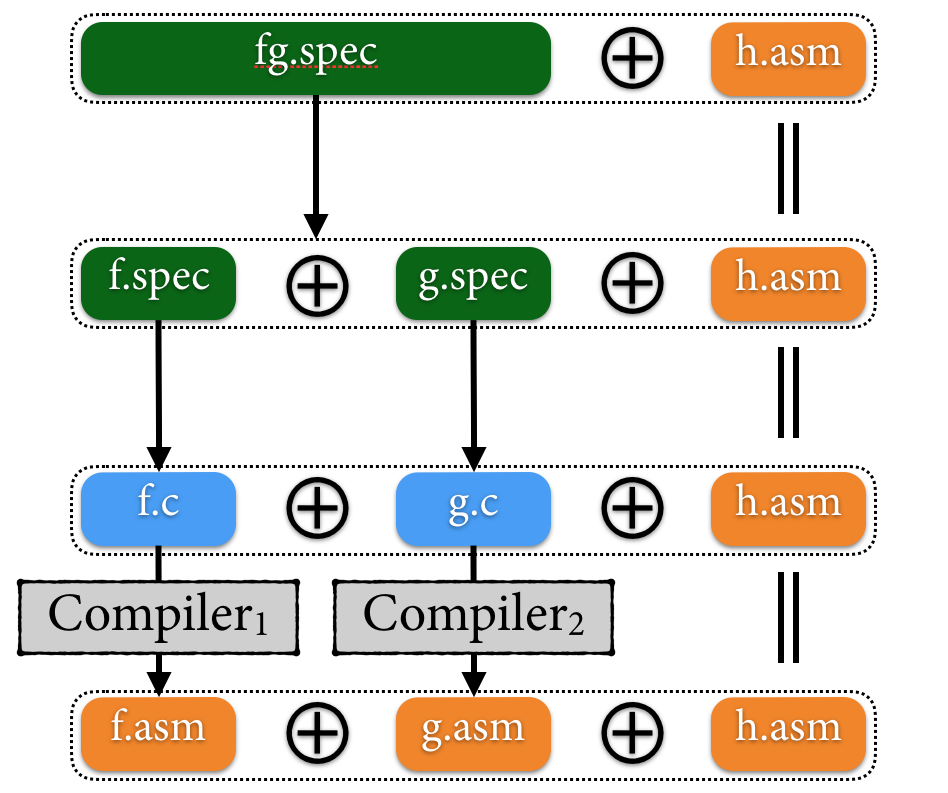
\includegraphics[width=0.90\linewidth]{images/program-verif.png}}
\caption{An end-to-end verification scenario}
\label{fig:program-verif}
\end{figure}



Now we explain how we can apply RUSC to program verification with an example (\Cref{fig:program-verif}) where two mutually recursive modules $\texttt{f.c}$ and $\texttt{g.c}$ are verified against its specifications even in the presence of an unknown assembly module $\texttt{h.asm}$.

First, we write a specification as a {\it module}, not in C but in abstract mathematical state transition system. %%simpler, abstract
For an instance, if we have a C module computing Fibonacci number employing dynamic programming technique, its specification module directly returns $\mathrm{Fib}(\code{n})$ for an argument \code{n} where $\mathrm{Fib}$ is a Gallina function.
Existing works\cite{lorch:armada, jung:irisjfp, VST, gu:dscal} often take different choice with us, where they write specifications in a specific language, as a {\it Hoare triple}, or as a CAL.
We use state transition system because it is the most general form, and fortunately it is already supported in interaction semantics. %% TODO: compare with multi-language semantics?

Then, each implementation module (written in C or assembly) is verified against its specification module using open simulations, thus implying RUSC relation.
The challenge here is: How to utilize the specifications of other modules even though what we are proving is RUSC, which quantifies over an arbitrary context?
Our key idea is that, instead of directly assuming the specifications of other modules, we carefully massage each specification module with UB in order to give an illusion as if we are assuming specifications of other modules.
Specifically, $\texttt{f.spec}$ calls $\texttt{g}$ -- which can be an arbitrary function because we are proving under an arbitrary context -- and then check if $\texttt{g}$ returns the expected value. If so, it will proceed, but if not, it will trigger UB.
As a result, when verifying $\texttt{f.spec} \rusc_\rels \texttt{f.c}$ one needs to proceed the simulation proof only when $\texttt{g}$ behaves as expected, because otherwise the proof is trivial.
After each module's verification is over, we can {\it merge} these modules to form $\texttt{fg.spec}$ and remove the potential source of UB.
This way, we can handle cooperation among the modules naturally.

Finally, recall that RUSC lifts (almost) arbitrary open simulations.
Therefore, even though verifying $\texttt{f.c}$ againts $\texttt{f.spec}$ requires a specialized simulation, RUSC can ably support them.

%%% 우리가 어떻게 하는지 설명
%%% hoare logic 단점들이랑 비교 -- 왜 그런 단점이 생겼나까지 설명할 필요는 없음.
%%% compiler verif랑 스타일 맞추려면... key challenge?

We demonstrate RUSC's potential as a program verification framework with interesting
examples, for which we write mathematical specifications as abstract
modules in interaction semantics and prove refinement between the
examples and their specification modules.  Specifically, we develop:
%% We have applied our idea to verify the following examples:
\begin{itemize}
\item Verification of \texttt{utod}: providing a correctness proof
  against its specification module using an open simulation,
  %% with the original memory injection,
  where \texttt{utod} is a handwritten
  assembly function casting unsigned long to double, whose correctness
  against its specification is axiomatized in \cc{} but not any more
  in \ccm{}.
  % (see \Cref{sec:utod-verification} for details).
\item \texttt{mutual-sum}: an example consisting of $(i)$ C and
  handwritten assembly modules that mutually recursively compute
  summation up to a given integer, performing memoization using
  module-local static variables, and $(ii)$ correctness proofs
  against their specification modules using open simulations with the
  new memory relation, memory injection with module-local invariants;
\end{itemize}
\medskip

%% Although the results are promising, RUSC as a program verification technique is still on its early stage and we will discuss future research directions in \todo{\ref{TODO}}.
%% Achieving high level of automation

Our approach is promising -- it does not suffer from a few drawbacks of higher-order separation logic -- but is still on early stage and further research is needed.
Specifically, we give clean and understandable specifications, prove total correctness, and our results are sound under arbitrary context, but our verification overhead is relatively higher than that of higher-order separation logic.
We will give a more comprehensive comparison in \Cref{sec:program:hoare} and discuss future research directions in \Cref{sec:program:future}.



%% First, we extend
%% The most advanced variants of Hoare logic today are ``higher-order concurrent separation logic''.
%% As the name implies,
%% As discussed above, using RUSC as a program verification technique shows promising results but its verification overhead is relatively high.
%% As discussed above, using RUSC as a program verification technique shows promising results but further research is needed to lower the verification overhead.
%% Specifically, modern extension of 
%% The reason is twofold. First, unlike compiler verification, program verification needs
%% interaction tree as a language

%Despite the promising results, verification overhead of our approach is relatively high, so further research is needed. %to lower the verification overhead.
%%% program verification 에서만 문제가 있고 compiler verification 과는 다르다는 것을 좀 더 이야기해야 함




%% variant separation logic, -- 지금 mutual sum도 Hoare style이라고 우길 수 있을 듯
%% Separation Logic
%% Future work: resource . pattern .
%% \todo{}
%% \todo{future works: separation logic is good (resource algebra) - and pattern/automation}

\bigskip
All our results are formalized in Coq, and it is available at: \[ \text{\url{https://sf.snu.ac.kr/compcertm}} \]

%% The remainder of the dissertation is structured as follows.
%% We give a high-level overview of the main ideas in
%% \Cref{sec:overview-verification}-\Cref{sec:overview-modulelocal};
%% the main results of \ccm{} and an analysis of its development in \Cref{sec:results};
%% its formal details in \Cref{sec:main-semantics}-\Cref{sec:main-verification};
%% and a comparison to related work in \Cref{sec:related}.
